% This is samplepaper.tex, a sample chapter demonstrating the
% LLNCS macro package for Springer Computer Science proceedings;
% Version 2.20 of 2017/10/04
%
\documentclass[runningheads]{llncs}
%
\usepackage{graphicx}
% Used for displaying a sample figure. If possible, figure files should
% be included in EPS format.
%
% If you use the hyperref package, please uncomment the following line
% to display URLs in blue roman font according to Springer's eBook style:
% \renewcommand\UrlFont{\color{blue}\rmfamily}

\begin{document}
%
    \title{Solving a skill labyrinth using Reinforcement Learning with Unity ML-Agents and Curriculum Learning}
%
    \titlerunning{Comparing RL and Curriculum Learning using ML-Agents}
% If the paper title is too long for the running head, you can set
% an abbreviated paper title here
%
    \author{\textbf{Mario da Graca}}
%
    \authorrunning{M. da Graca}
% First names are abbreviated in the running head.
% If there are more than two authors, 'et al.' is used.
%
    \institute{
        \textsl{
            Self-optimizing Systems\\
            Winter Term 2022/23\\
            University of Applied Sciences (HAW Hamburg)\\
            Berliner Tor 5, 20999 Hamburg\\
        }
    }
%
    \maketitle              % typeset the header of the contribution
%
    \begin{abstract}
        This project report examines curriculum learning in Unity ML-Agents using a 3D skill labyrinth as an example.
        The task involves tilting the board on two axes to guide a marble through a labyrinth, filled with walls and holes, through which the agent must steer the marble in order to follow the correct path and reach the end.
        The agent's performance was evaluated using two different approaches: standard reinforcement learning and curriculum learning.
        Curriculum learning involves starting the agent with simpler sub-tasks, and gradually increasing the difficulty over time.
        The paper covers the technical details of the project, including setup of the environment, tuning of parameters, reward engineering and performance analysis of the trained agent.

        \keywords{Reinforcement Learning \and Curriculum Learning \and Unity ML-Agents}
    \end{abstract}

    %! Author = mario
%! Date = 25.01.2023

\section{Introduction}\label{sec:introduction}
Machine learning (ML) is a subset of Artificial Intelligence (AI) that focuses on the development of algorithms and statistical
models that allow computers to learn from data and make predictions or judgments without being explicitly programmed.
Reinforcement Learning is a type of Machine Learning that focuses on teaching agents to make decisions in a given environment
by maximizing a reward signal.
It is a method for an agent to learn how to behave in a given situation by executing specific
actions and watching the rewards that the environment provides.\\
ML and RL are widely used in a range of applications, such as robotics, autonomous vehicles, finance, healthcare and games.
This report explores Reinforcement Learning in the latter one, by creating a complex and agility focused labyrinth environment,
that an agent has to successfully solve.
With the help of Unity's ML-Agents~\cite{juliani2020} a model is trained using the standard Reinforcement Learning and Curriculum Learning~\cite{narvekar_learning_2018} approach.
The goal of this project was to explore the process of an agent learning a fine motor task.
The following chapter will explain the setup of the board game in real life and as a game in the Unity engine~\cite{Haas2014AHO} to lay the grounds
for the third chapter, where the reinforcement learning aspects of this project are described.
The focus is on the environment and training setup, as well as the reward engineering.
In chapter four the used metrics are discussed and the results presented, in order to give a qualified statement in chapter five
about the performances and show where the process can be improved.

    %! Author = mario
%! Date = 30.01.2023


\section{Game Implementation}\label{sec:game-implementation}

\subsection{Game board}\label{subsec:game-board}
The basic setup of the game is simple, yet the hard parts lie in the way the game is played.
As shown in Fig.~\ref{fig:wooden_board} the game board is made out of wood and tilt-able on two disconnected axes.
This allows the player to move the marble around without direct contact, just by leveraging gravitation.
The goal of this game is to reach the end on the right hand side of the board, without falling into a hole.
If the marble falls down, the player has to restart and is rewarded with the points that are associated with each hole.
To follow the rules, the marble has to pass the holes in the correct order given by the black line.
Only if these requirements are met, the player can win the game.
There is no time limit in this game.\\
The basic concepts are easy to learn, but solving the task is hard to master.
The game requires fine adjustments to the angles and quick reactions to prevent the marble from rolling uncontrolled through
the labyrinth.

\begin{figure}[h]
    \centering
    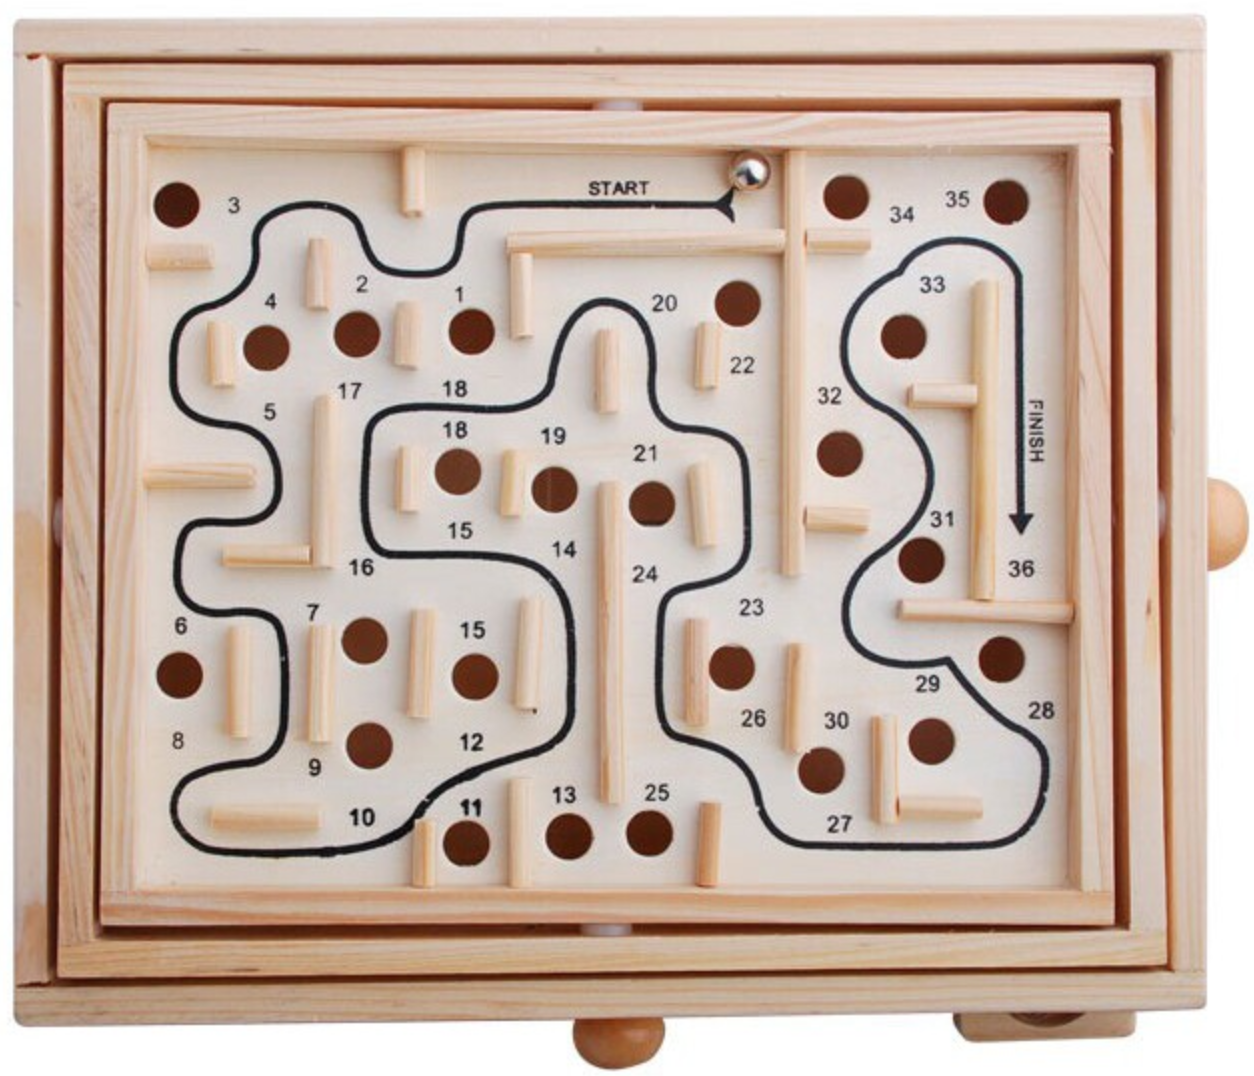
\includegraphics[width=0.65\textwidth]{images/wooden_game_board}
    \caption{The wooden game board, with the path to follow. Source:~\cite{wooden_board}}
    \label{fig:wooden_board}
\end{figure}

\subsection{Unity game board}\label{subsec:unity-game-board}
To closely approximate the movement and behavior of the marble in this physics based skill game,
Unity's built-in physics engine (PhysX3).
This system provides several components that can be attached to game objects, to ensure specific behaviors.
A game object in Unity defines the base for any entity in the given scene.
\begin{itemize}
    \item{Collider3D}: The Collider3D component can be added to any game object, either static or dynamic, to simulate the contact points of hard surfaces, like the marble or the game board.
    The shape is usually defined by or similar to the actual 3D model.
    This component can serve two purposes.
    It either behaves like a collider or, if specified by a flag, acts as a trigger, meaning it's not bouncing off other game objects.
    Instead it sends out a trigger signal.
    \item{Rigidbody3D}: To add game objects to the physics simulation that are affected by gravity, the Rigidbody3D component with the associated flag can be added to game objects with a Collider3D.
\end{itemize}
With these two simple components and a C\# script the controls and gameplay can be simulated.\\
In addition to the original game board, some modifications had to be made:
\begin{enumerate}
    \item{Top cover}: To make sure that the marble can't bounce out of the labyrinth, a transparent Collider3D has been
    added as a lid on top of the labyrinth.
    \item{Holes}: The board has holes in the base plate in the same positions as the original game board.
    Another Collider3D, but as a trigger, has been added below the game board to know, when the marble has fallen through a hole.
    The game will reset, if this event occurs.
    \item{Checkpoints}: Since the rules state that the marble has to follow the given path a checkpoint system has been implemented to ensure that the agent learns the correct behavior.
    A marble can only pass through the current checkpoint in line, otherwise the game will reset.
\end{enumerate}


    \clearpage
    \bibliographystyle{splncs04}
    \bibliography{references}
%
\end{document}
